\chapter{Statistics}
\label{chap:stat}

% move the ML/MM stuff here, with ex of a random effects model of mean
% ratings within users

% then the other ML/MM leave in the stat recysys chapter

It is assumed here that the reader has background in basic statistical
inference, i.e.\ hypothesis testing and confidence intervals.

\section{Sample vs.\ Population}

Most readers have probably noticed that when the results of a survey are
released, say during elections, a \textit{margin of error} (MOE) is stated.
For instance, ``55\% of those surveyed say they plan to vote for
Candidate Jones, with a margin of error of 3.2\%.''  The MOE is
recognition of the fact that only a sample of voters were surveyed, not
the entire population of voters.

Let $p$ denote the population proportion, i.e.\ the proportion of voters
across the population who favor Jones.  The value of $p$ is unknown, but
our estimate is $\widehat{p} = 0.55$.

Assuming the voters were polled at random, $\widehat{p}$ is a random
variable.  As such, it has a standard deviation, which can be shown to
be

\begin{equation}
[p(1-p)/n] ^{0.5}
\end{equation}

which we in turn estimate as

\begin{equation}
[\widehat{p}(1-\widehat{p})/n] ^{0.5}
\end{equation}

where $n$ is th number of people polled.  This is the \textit{standard
error} of $\widehat{p}$, and is a measure of how accurate $\widehat{p}$
is as an estimate of $p$.

What about the MOE?  This is 1.96 times the standard error, and is the
radius of an approximate 95\% confidence interval for $p$.

Every ML method is an estimator in some form or other.  However,
the terms \textit{sample} and \textit{population} are not used in the ML
community.  Instead, they speak a \textit{generative process} to mean
the same thing as sampling data from a population.

\section{How Do We Select an Estimator?}

\subsection{Sample Analogs}

In our survey example above, our estimate $\widehat{p}$ is the sample
analog of the population value $p$; the former is the proportion in our
sample data and the latter is the proportion in the population.

Similarly, say we wish to estimate a population variance, say the
variance of blood pressure $Var(B)$ in some patient population.  The
sample analog is

\begin{equation}
\label{s2}
s^2 = \frac{1}{n} \sum_{i=1}^n (B_i - \overline{B})^2
\end{equation}

where the $B_i$ are the blood pressures in our sample, and $\overline{B}$
is the average pressure in our sample.  This is analogous to the
population value,

\begin{equation}
Var(B) = E[(B - EB)^]
\end{equation}

How about estimating a covariance matrix?  Again, an extension of
(\ref{s2}).  Say our sample consists of $n$ vectors
$U_1,...,U_n$.  Then

\begin{equation}
\widehat{Cov}(U) =
\frac{1}{n}
\sum_{i=1}^n (U_i - \overline{U}) (U_i - \overline{U})'
\end{equation}

where here $\overline{U}$ is the average of the \textit{vectors} $U_i$.

In many cases, the choice of estimator is less straightforward.  For
instance, say we wish to estimate the probability density of $B$, 
$f_B()$.  Actually, you already know such an estimator---a histogram!
As long as one scales to histogram to have total area 1.0 (in R's
\lstinline{hist()} function, set \lstinline{probability=TRUE}), this
provides an estimate of $f_B()$.  Let's call the histogram
$\widehat{f}_B()$.

\subsection{Consistency of Estimators}

What do we mean in saying that an estimator is an estimate of something?
At the very least, we should require \textit{consistent}, meaning that
the estimator converges to the population quantity as the sample size
grows.

For example, in the survey example, we have 

\begin{equation}
\lim_{n \rightarrow \infty} \widehat{p} = p
\end{equation}

But what about the histogram case?  For the estimator to be consistent,
we need not only $n \rightarrow \infty$ but also $h \rightarrow 0$,
where $h$ is the bin width.\footnote{Technically, we cannot allow $h$
to go to 0 ``too quickly,'' but this issue is beyond the scope of this
book.}

\subsection{Unbiasedness of Estimators}

Another classical criterion for goodness of an estimator is that it be
\textit{unbiasded}, which means the expected value of the estimator is
the population quantity.  In the survey example above, this criterion
would ask that

\begin{equation}
E\widehat{p} = p
\end{equation}

which in fact can be shown to be true.

But $s^2$ is more complicated.  Books typically divide by $n-1$ instead
of $n$ in (\ref{s2}), as a ``fudge factor'' to make

\begin{equation}
E(s^2) = \sigma^2
\end{equation}

where the right-hand side denotes the population variance.  But actually 
even with the fudge factor $s$ (without the power 2) is biased:

\begin{equation}
0 < Var(s) = E(s^2) - (Es)^2 = \sigma^2  - (Es)^2 
\end{equation}

so

\begin{equation}
Es < \sigma
\end{equation}

rather than

\begin{equation}
Es = \sigma
\end{equation}

At the time basic statistics was being developed---about 100 years
ago---not much was known, so unbiasedness was considered important.
It in fact is still useful in some settings, but today it's understood 
that we should not emphasize it so much.

Indeed, a big issue in ML is the Bias-Variance Tradeoff.  In the above
context, dividing by $1/n$ instead of $1/(n-1)$ reduces variance, 
i.e.\ reduces $Var(s^2)$, which is good, at a cost of increasing bias, a
tradeoff.

Actually, it can be shown that the best mean squared error for $s^2$
comes from dividing by $1/(n+1)$.  We'll use $n$ here to keep the
analogy tight.  Of course, for large $n$, the difference is negligible.

\subsection{Fitting Parametric Models}

It is often the case that one may try to fit a parametric family of
densities to one's datat.  Let's use MovieLens as an example.

\begin{lstlisting}
> nu <- ml100kpluscovs$Nuser
> hist(nu)
\end{lstlisting}

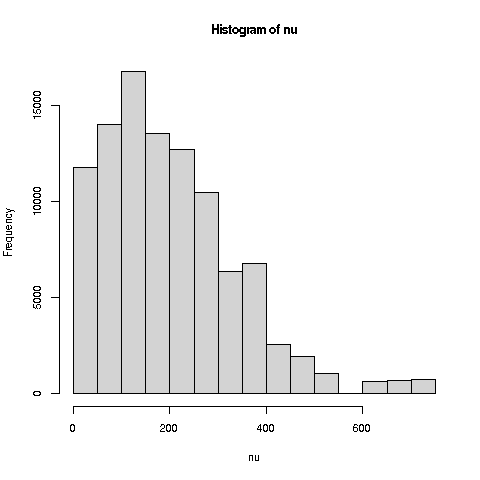
\includegraphics[width=3.5in]{Images/NuserGamma.png}

That shape seems to suggest a good fit from the \textit{gamma} family of
densities,

\begin{equation}
\label{erlang}
f_{W}(t) = \frac{1}{(r-1)!} \lambda^r t^{r-1} e^{-\lambda t}, ~ t > 0
\end{equation}

A typical curve looks something like this:

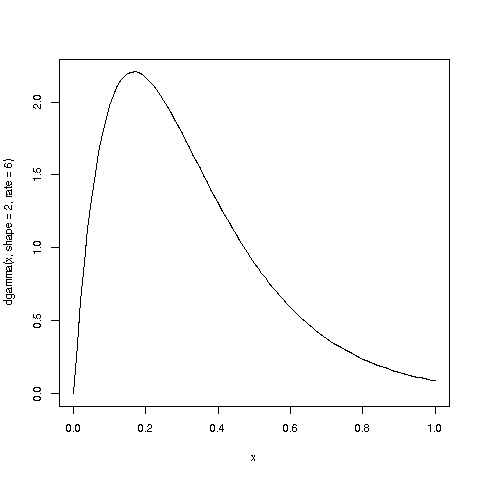
\includegraphics[width=3.0in]{Images/ErlangShape2Rate6.png}

The family has parameters $r$ and $\lambda$.\footnote{Technically this
is a subset of the gamma family, called \textit{Erlang}, but the only
restriction is that $r$ be an integer.}  For each value of the latter
two quantities, we get a different curve, some flatter, some more
peaked.

The question at hand is:

\begin{quote}
Is there some $(r,\lambda)$ pair such such that the curve (\ref{erlang})
fits the data well?
\end{quote}

The task is then to:

\begin{itemize}

\item Estimate $r$ and $\lambda$ from our data.

\item Check the fit.

\end{itemize} 

How do we do the estimation?  Two standard methods are the Method of
Moments (MM) and Method of Maximum Likelihood (MLE).

\subsubsection{The Method of Moments}

The idea is simple, at least in concept.  Here's how it works in the
gamma example above.

First, some terminology:  For a random variable $X$, the $k^{th}$
\textit{moment} is $E(X^k),~ k=1,2,3,...$.  A variant is the $k^{th}$
\textit{central moment}, $E[(X - EX)^k]$.  Either the ordinary or
central moments are fine.

Let $N$ denote the number of ratings.  Then for the gamma family,

\begin{equation}
EN = r/\lambda
\end{equation}

and

\begin{equation}
Var(N) = r/\lambda^2
\end{equation}

Then replace everything by sample analogues:

\begin{equation}
\overline{X} = \widehat{r} / \widehat{\lambda}
\end{equation}

and

\begin{equation}
s^2 = \widehat{r} / \widehat{\lambda}^2
\end{equation}

Dividing the first equation by the second, we obtain

\begin{equation}
\widehat{\lambda} = \overline{N} / s^2
\end{equation}

and thus from the first equation,

\begin{equation}
\widehat{r} = \overline{N} \widehat{\lambda} = \overline{N}^2 / s^2
\end{equation}

where $ \overline{N}$ and $s^2$ are the sample mean and variance of
$N_1,...,N_n$ for $n$ users.

Now, what about assessing the fit?  A classic method is a
\textit{goodness of fit test}, but these days hypothesis testing is
frowned upon, for good reason.  Here's why:

